%%%%%%%%%%%%%%%%%%%%%%%%%%%%%%%%%%%%%%%%%
% a0poster Landscape Poster
% LaTeX Template
% Version 1.0 (22/06/13)
%
% The a0poster class was created by:
% Gerlinde Kettl and Matthias Weiser (tex@kettl.de)
% 
% This template has been downloaded from:
% http://www.LaTeXTemplates.com
%
% License:
% CC BY-NC-SA 3.0 (http://creativecommons.org/licenses/by-nc-sa/3.0/)
%
%%%%%%%%%%%%%%%%%%%%%%%%%%%%%%%%%%%%%%%%%

%----------------------------------------------------------------------------------------
%	PACKAGES AND OTHER DOCUMENT CONFIGURATIONS
%----------------------------------------------------------------------------------------

\documentclass[a0,landscape]{a0poster}

\usepackage{multicol} % This is so we can have multiple columns of text side-by-side
\columnsep=100pt % This is the amount of white space between the columns in the poster
\columnseprule=3pt % This is the thickness of the black line between the columns in the poster

\usepackage[svgnames]{xcolor} % Specify colors by their 'svgnames', for a full list of all colors available see here: http://www.latextemplates.com/svgnames-colors

\usepackage{times} % Use the times font
%\usepackage{palatino} % Uncomment to use the Palatino font

\usepackage{graphicx} % Required for including images
\graphicspath{{figures/}} % Location of the graphics files
\usepackage{booktabs} % Top and bottom rules for table
\usepackage[font=small,labelfont=bf]{caption} % Required for specifying captions to tables and figures
\usepackage{amsfonts, amsmath, amsthm, amssymb} % For math fonts, symbols and environments
\usepackage{wrapfig} % Allows wrapping text around tables and figures
\usepackage{enumitem}
\usepackage{listings}% http://ctan.org/pkg/listings
\lstset{
  basicstyle=\ttfamily,
  mathescape
}
\usepackage{pgf,tikz}
\usepackage{pgfplots}
\pgfplotsset{compat=newest}

\DeclareMathOperator{\rank}{rank}
\DeclareMathOperator{\spann}{span}
\newcommand\SPAN[1]{\ensuremath\spann(#1)}

\newtheorem{thm}{Theorem}
\newtheorem{lemma}{Lemma}
%\newtheorem{proposition}{Proposition}
\newtheorem{coro}{Corollary}
%\newtheorem{definition}{Definition}
\newtheorem{remark}{Remark}

\begin{document}

%----------------------------------------------------------------------------------------
%	POSTER HEADER 
%----------------------------------------------------------------------------------------

% The header is divided into three boxes:
% The first is 55% wide and houses the title, subtitle, names and university/organization
% The second is 25% wide and houses contact information
% The third is 19% wide and houses a logo for your university/organization or a photo of you
% The widths of these boxes can be easily edited to accommodate your content as you see fit

\begin{minipage}[b]{0.58\linewidth}
  \veryHuge \color{NavyBlue} \textbf{Incremental SVD Algorithms} \color{Black}\\ % Title
  \Huge\textit{For Distributed Analysis of Agglomerative Data on Large Networks}\\[1cm] % Subtitle
  \huge \textbf{Benjamin W.~Ong \quad \& \quad Mark A.~Iwen}\\ % Author(s)
  \huge Michigan Tech \hspace*{3.2in} Michigan State University\\ % University/organization
\end{minipage}
%
\begin{minipage}[b]{0.22\linewidth}
  \Large \textbf{Contact Information:}\\
  Benjamin W.~Ong\\
  Michigan Technological University\\
  Department of Mathematical Sciences \\
  Houghton, MI\\\\
  Email: \texttt{ongbw@mtu.edu}\\ % Email address
\end{minipage}
%
\begin{minipage}[b]{0.19\linewidth}
  
\includegraphics[width=20cm]{figures/logo.png} % Logo or a photo of you, adjust its dimensions here\\
  \vspace*{2in}
\end{minipage}

\vspace{1cm} % A bit of extra whitespace between the header and poster content

%----------------------------------------------------------------------------------------

\begin{multicols}{4} % This is how many columns your poster will be broken into, a poster with many figures may benefit from less columns whereas a text-heavy poster benefits from more

%----------------------------------------------------------------------------------------
%	ABSTRACT
%----------------------------------------------------------------------------------------

\begin{abstract}
  We show that the SVD of a matrix can be constructed efficiently in a
  hierarchical approach. The proposed algorithm is proven to recover
  the singular values and left singular vectors of the input matrix 
  if its rank is known. Further, the hierarchical algorithm can be
  used to recover the largest singular values and left singular
  vectors with bounded error. It is also shown that the proposed
  method is stable with respect to roundoff errors or corruption of
  the original matrix entries. Numerical experiments validate the
  proposed algorithms and parallel cost analysis.
\end{abstract}

%----------------------------------------------------------------------------------------

\section*{Motivation}
\begin{itemize}[noitemsep]
\item The SVD algorithm is widely used for principal component
  analysis and low-rank approximations.
\item We are interested in streaming data.  Suppose $A$ is known, $B$
  is data which is yet to arrive.  If $A=U\Sigma V'$ is already
  computed, we wish to utilize factorization to compute the SVD
  decomposition of $[A\, B]$.
\item Tackle big (volume) distributed streaming data.
\end{itemize}

\section*{Idea}

One-level distributed SVD algorithm:
\begin{center}
  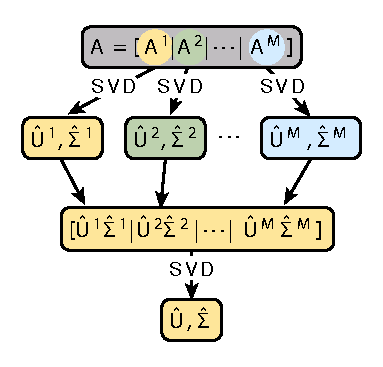
\includegraphics[width=0.55\linewidth]{figures/tikz_one_level_flowchart}
  \captionof{figure}{Different colors: different
    processors completing operations in parallel.}
\end{center}\vspace{1cm}

Two-level distributed SVD:
\begin{center}
  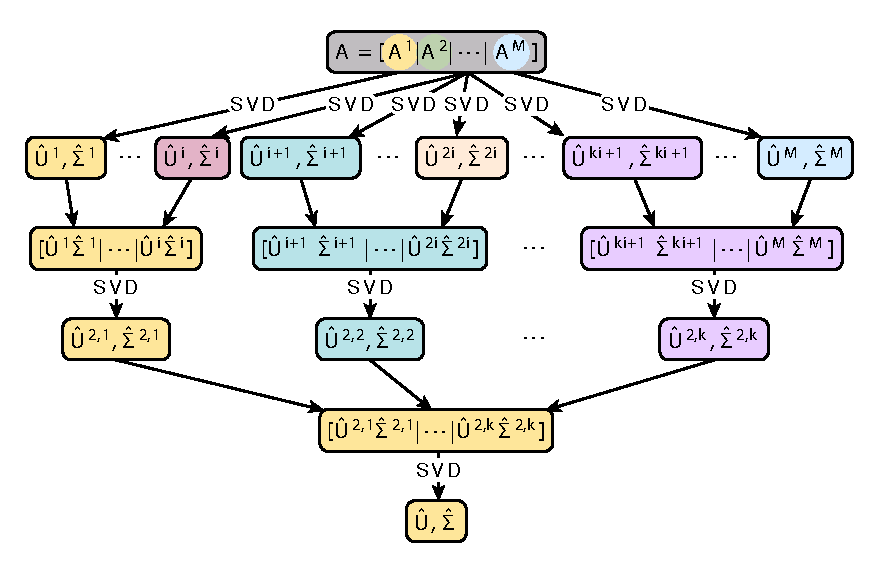
\includegraphics[width=1.05\linewidth]{figures/tikz_two_level_flowchart}
  \captionof{figure}{Different colors: different
    processors completing operations in parallel.}
\end{center}\vspace{1cm}

\section*{Algorithm}
Input:
\begin{itemize}[noitemsep]
\item $q$: number of levels
\item $n$: \# local SVDs to concatenate at each level
\item $d$: intrinstic dimension, $d\in\{1,\ldots,D\}$
\item $A^{1,i} := A^i \in \mathbb{C}^{D\times N_i},\,$ 
  $i=1,2,\ldots,M$ (block decomposition of $A$)
\end{itemize}
Output:
\begin{itemize}[noitemsep]
\item $U' \in \mathbb{C}^{D \times d} \approx$ the first $d$
  columns of $U$;
\item $\Sigma' \in \mathbb{R}^{d \times d} \approx \left(\Sigma
  \right)_d$.
\end{itemize}
\hrulefill
\begin{lstlisting}
for p = 1..q
  Compute (in parallel), $A^{p,i} = U^{p,i} \Sigma^{p,i}  \left( V^{p,i} \right)^*$
                         $i=1,2,\ldots,M / n^{(p-1)}$

  Set $\displaystyle A^{p+1,i} := \left[ \left( U^{p,(i-1)n+1} \Sigma^{p,(i-1)n+1} \right)_d ~\Big| \cdots \Big|~ \left( U^{p,in} \Sigma^{p,in} \right)_d \right]$
                         $i=1,2,\ldots,M / n^p$.

end

Compute the SVD of $A^{q+1,1}$

Return $U' :=$ the first $d$ columns of $U^{q+1,1}$, and
       $\Sigma':= \left( \Sigma^{q+1,1} \right)_d$
\end{lstlisting}
\hrulefill

\vspace*{-0.5in}
\section*{Numerics}
Strong scaling study:
\begin{center}
  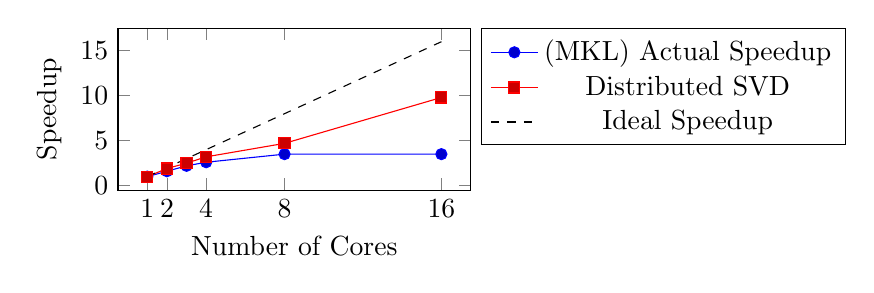
\begin{tikzpicture}
    \begin{axis}[
        xlabel={Number of Cores},
        xtick={1,2,4,8,16},
        yminorticks=true,
        legend pos = outer north east,
        ylabel={Speedup},
        width=0.5\linewidth,
        height=0.3\linewidth
      ]
      
      \addplot coordinates {
        (1, 1)
        (2, 1.6)
        (3, 2.2)
        (4, 2.6)
        (8, 3.5)
        (16, 3.5)
      };
      \addlegendentry{(MKL) Actual Speedup}
      
      \addplot coordinates {
        (1, 1)
        (2, 1.9)
        (3, 2.5)
        (4, 3.2)
        (8, 4.7)
        (16, 9.8)
      };
      \addlegendentry{Distributed SVD}
      
      \addplot [color=black,dashed] coordinates {
        (1, 1)
        (2, 2)
        (4, 4)
        (8, 8)
        (16, 16)
      };
      \addlegendentry{Ideal Speedup}
    \end{axis}
  \end{tikzpicture}
  \captionof{figure}{Strong scaling study of the {\tt dgesvd} function in the
    threaded Intel MKL library (blue) and the proposed distributed SVD
    algorithm (red).  The input matrix is of size
    $2000\times1,152,000$.  }
\end{center}
Weak scaling study:
\begin{center}
  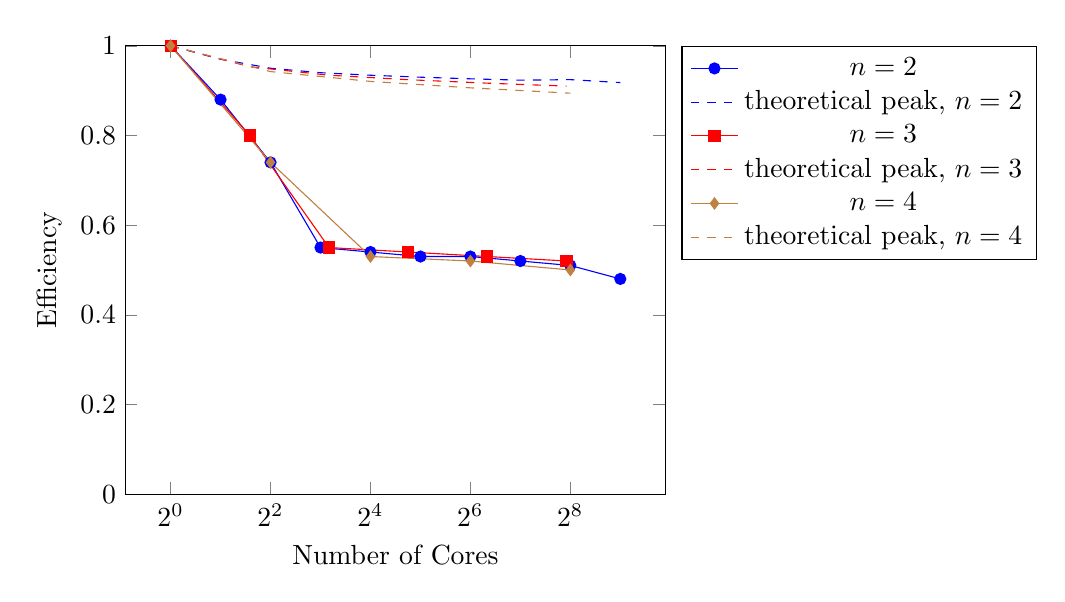
\begin{tikzpicture}
    \begin{semilogxaxis}[
        xlabel={Number of Cores},
        yminorticks=true,
        legend pos = outer north east,
        ylabel={Efficiency},
        ymin=0,
        ymax=1,
        log basis x={2}]]
        
        \addplot[mark=oplus*, color=blue] coordinates {
          (1, 1)
          (2, 0.88) 
          (4, 0.74)
          (8, 0.55)
          (16, 0.54)
          (32, 0.53)
          (64, 0.53)
          (128, 0.52)
          (256, 0.51)
          (512, 0.48)
        };
        \addlegendentry{$n=2$}
        
        \addplot[mark=none,style=dashed,color=blue] coordinates {
          (1,1)
          (2,1.94/2)
          (4,3.80/4)
          (8,7.52/8)
          (16, 14.95/16)
          (32,29.76/32)
          (64, 59.29/64)
          (128,118.19/128)
          (256,236.68/256)
          (512,470.00/512)
        };
        \addlegendentry{theoretical peak, $n=2$}

        \addplot [mark=square*,color=red] coordinates {
          (1, 1)
          (3, 0.8)
          (9, 0.55)
          (27,0.54)
          (81, 0.53)
          (243, 0.52)
        };
        \addlegendentry{$n=3$}


        \addplot [mark=none,style=dashed,color=red] coordinates {
          (1, 1)
          (3, 2.86/3)
          (9, 8.41/9)
          (27, 24.96/27)
          (81, 74.25/81)
          (243, 221.15/243)
        };
        \addlegendentry{theoretical peak, $n=3$}      

        \addplot [mark=diamond*,color=brown] coordinates {
          (1, 1)
          (4, 0.74)
          (16, 0.53)
          (64, 0.52)
          (256, 0.50)
        };
        \addlegendentry{$n=4$}
        
        \addplot [mark=none,color=brown, style=dashed] coordinates {
          (1, 1)
          (4, 3.77/4)
          (16, 14.73/16)
          (64, 58.00/64)
          (256, 228.94/256)
        };
        \addlegendentry{theoretical peak, $n=4$}
        
    \end{semilogxaxis}
  \end{tikzpicture}
  \captionof{figure}{The input matrix is of size $2000\times (32000
    M)$, where $M$ is the processing cores used in the computation.
    The intrinsic dimension is $d=200 \ll 2000$.  The observed
    efficiency is plotted for various $n$'s (number of scaled singular
    vectors concatenated at each hierarchical level).}
\end{center}


\subsection*{Mathematical Preliminaries}
Let $A \in \mathbb{C}^{D \times N}$ be a highly rectangular matrix,
with $N \gg D$.  Further, let $A^i \in \mathbb{C}^{D\times N_i}$ with
$i=1,2,\ldots,M$, denote the block decomposition of $A$, i.e.,
$A=\left[A^1|A^2|\cdots|A^M\right]$.

\begin{itemize}[noitemsep]
\item For any matrix $A \in \mathbb{C}^{D \times N}$, $(A)_d\in
  \mathbb{C}^{D \times N}$ is an optimal rank $d$ approximation to $A$
  with respect to Frobenius norm $\| \cdot \|_{\rm F}$ if
  \begin{align*}
    \inf_{B\in \mathbb{C}^{D\times N}} \|B-A\|_F = \|(A)_d - A\|_F,
    \text{ subject to } \rank{(B)} \le d.
  \end{align*}

\item If $A$ has the SVD decomposition $A = U\Sigma V^*$, then $(A)_d
= \sum_{i=1}^d u_i \sigma_i v_i^*$, where $u_i$ and $v_i$ are singular
vectors that comprise $U$ and $V$ respectively, and $\sigma_i$ are
the singular values.

\item The Frobenius norm can be computed using $ \|A\|^2_F = \sum_i^D
  \sigma_i^2$ Consequently, $ \|(A)_d - A \|^2_F = \sum_{d+1}^D
  \sigma_i^2$.
  
\end{itemize}



\section*{Analysis}
We show that the hiearchical SVD algorithm can recover the $d$ largest
singular values and left singular vectors with bounded error.  We also
show that the proposed method is stable with respect to roundoff
errors or corruption of the original matrix entries.
\begin{lemma}
  Suppose $A^i \in \mathbb{C}^{D\times N_i}, i=1,2,\ldots,M$.
  Further, suppose matrix $A$ has block components
  $A=\left[A^1|A^2|\cdots|A^M\right]$, and $B$ has block components
  $B=\left[(A^1)_d | (A^2)_d |\cdots|(A^M)_d \right]$.  Then, $$\|
  (B)_d - A \|_{\rm F} \leq \| (B)_d - B \|_{\rm F} +  \| B - A \|_{\rm F} \leq 3 \| (A)_d - A \|_{\rm F}$$ holds for all $d \in \{ 1, \dots, D\}$.
\end{lemma}


\begin{thm}
  Suppose that $A \in \mathbb{C}^{D\times N}$ has block components
  $A^i \in \mathbb{C}^{D\times N_i}, i=1,2,\ldots,M$, so that
  $A=\left[A^1|A^2|\cdots|A^M\right]$.  Let
  $B=\left[\overline{(A^1)_d} ~\big|~ \overline{(A^2)_d} ~\big|~
    \cdots~\big|~ \overline{(A^M)_d} \right]$, $\Psi \in
  \mathbb{C}^{D\times N}$, and $B' = B + \Psi$.  Then, there exists a
  unitary matrix $W$ such that
  $$\left\| \overline{\left( B' \right)_d} - AW \right\|_{\rm F} \leq
  3\sqrt{2} \| (A)_d - A \|_{\rm F} + \left(1+ \sqrt{2} \right) \|
  \Psi \|_{\rm F}$$ holds for all $d \in \{ 1, \dots, D\}$.
\end{thm}

\begin{thm}
  Let $A \in \mathbb{C}^{D\times N}$ and $q \geq 1$.  Then, the
  hierarchical SVD merging algorithm is guaranteed to recover an
  $A^{q+1,1} \in \mathbb{C}^{D\times N}$ such that
  $\overline{\left(A^{q+1,1} \right)_d} = A W + \Psi$, where $W$ is a
  unitary matrix, and $\| \Psi \|_{\rm F} \leq \left( \left( 1 +
  \sqrt{2} \right)^{q+1} - 1 \right) \| (A)_d - A \|_{\rm F}$.
\end{thm}

\begin{thm}
  Let $\alpha$ and $\beta$ respectively represent the latency cost and
  the transmission cost of sending a floating point number between two
  processors.  The parameter $\gamma$ represents the time for one
  floating point operation (FLOP).  The communication cost for the
  hierarchical SVD algorithm is
  \begin{align*}
    q\left(\alpha  + d\,(n-1)\,D\beta\right).
  \end{align*}
  The potential parallel speedup satisfies:
  \begin{align*}
  \frac{(2 ND^2 + 2 D^3)\gamma} {\gamma\left[(2 (N/M)D^2 + 2D^3) + q(2dnD^2
      + 2D^3)\right] +q (\alpha + d(n-1)D\beta)},
  \end{align*}
  if $ nd > D$, and 
  \begin{align*}
    \frac{(2 ND^2 + 2 D^3)\gamma} {\gamma\left[(2 (N/M)D^2 + 2D^3) + q(2(dn)^2D
        + 2(dn)^3)\right] +q (\alpha + d(n-1)D\beta)},
  \end{align*}
  otherwise.
\end{thm}
\noindent The proofs and supporting lemmas are found in the manuscript
\cite{doi:10.1137/16M1058467}.

\section*{Discussion/Open Problems}
\begin{itemize}[noitemsep]
\item The right singular vectors can be computed (in parallel) if
  desired, once the left singular vectors and singular values are
  known.  The master process broadcasts the left singular vectors and
  singular values to each process containing block $A^i$.  Then
  columns of the right singular vectors can be constructed by
  computing $\frac{1}{\sigma_j}(A^i)^* u_j$, were $A^i$ is the block
  of $A$ residing on process $i$, and $(\sigma_j,u_j)$ is the $j^{th}$
  singular value and left singular vector respectively.

\item To handle streaming data with time-varying characteristics, need
  ability to ``decrement'' factorization.  Possible with one-pass?
\item For sparse data, hierarchical merging algorithm not practical.
  Explore CUR decomposition?
\item Apply to spectral clustering?
\item Interested in multiscale construction of low-dimensioanl
  manifold using streaming data.
\end{itemize}
 %----------------------------------------------------------------------------------------
%	REFERENCES
%----------------------------------------------------------------------------------------
\nocite{*} % Print all references regardless of whether they were cited in the poster or not
\bibliographystyle{plain} % Plain referencing style
\bibliography{svd} % Use the example bibliography file sample.bib

%----------------------------------------------------------------------------------------
%	ACKNOWLEDGEMENTS
%----------------------------------------------------------------------------------------

\section*{Acknowledgements}
\begin{itemize}[noitemsep]
\item B.~W.~Ong was supported in part by AFOSR FA9550-12-1-0455.
\item M.~A.~Iwen was supported in part by NSF DMS-1416752 and NSF
  CCF-1615489.
\item This work utilized computational resources provided by superior,
  the high-performance computing cluster @ MTU, and by the Extreme
  Science and Engineering Discovery Environment (XSEDE), which is
  supported by National Science Foundation grant number ACI-1053575.
\end{itemize}

\vspace*{1in}
\end{multicols}
\end{document}
